\documentclass[aspectratio=169,11pt]{beamer}
% Light academic theme. Set2 colours are used for graphical accents.
\usepackage{fix-cm}
\usepackage[T1]{fontenc}
\usepackage[utf8]{inputenc}
\usepackage{amsmath,amssymb,booktabs,graphicx,tikz}
\usepackage{mathpazo}
\usepackage{bm}
\usepackage[default]{sourcesanspro}
\usefonttheme{professionalfonts}
\usetikzlibrary{arrows.meta,calc,positioning,patterns}
\definecolor{Paper}{HTML}{FCFBF8}
\definecolor{Ink}{HTML}{25333A}
\definecolor{Muted}{HTML}{59656A}
\definecolor{Rule}{HTML}{D5DAD8}
\definecolor{Green}{HTML}{66C2A5}
\definecolor{Orange}{HTML}{FC8D62}
\definecolor{Blue}{HTML}{8DA0CB}
\definecolor{Pink}{HTML}{E78AC3}
\definecolor{GreenText}{HTML}{28634F}
\definecolor{BlueText}{HTML}{465A81}
\setbeamercolor{normal text}{fg=Ink,bg=Paper}
\setbeamercolor{background canvas}{bg=Paper}
\setbeamercolor{math text}{fg=Ink}
\setbeamercolor{structure}{fg=GreenText}
\setbeamertemplate{navigation symbols}{}
\setbeamertemplate{headline}{}
\setbeamertemplate{footline}{}
\hypersetup{colorlinks=true,urlcolor=BlueText,linkcolor=Ink,
 pdftitle={Estimation of Quantum Fisher Information by variational quantum circuits on a quantum computer},
 pdfauthor={Luca Manzi},pdfsubject={Master's thesis defence; academic presentation}}
\input{glyphtounicode}
\pdfgentounicode=1
\pdfstringdefDisableCommands{\def\translate#1{#1}}
\graphicspath{{assets/}}
\newcommand{\MainSlideCount}{14}
\newenvironment{canvas}{\begin{tikzpicture}[remember picture,overlay,x=1cm,y=1cm]
 \begin{scope}[shift={(current page.south west)}]}{\end{scope}\end{tikzpicture}}
\tikzset{txt/.style={anchor=north west,align=left,inner sep=0pt,text=Ink,font=\normalsize},
 smalltxt/.style={txt,font=\small,text=Muted},
 eq/.style={txt,font=\fontsize{17}{21}\selectfont},
 arr/.style={-{Stealth[length=2.3mm]},line width=1pt,draw=Muted},
 flow/.style={draw=Rule,fill=white,minimum height=1cm,text=Ink,align=center,font=\small,text width=2.1cm,inner sep=5pt}}
\newsavebox{\titlebox}
\newcommand{\fittitle}[1]{\sbox{\titlebox}{\rmfamily\fontsize{23}{27}\selectfont #1}%
 \ifdim\wd\titlebox>14.3cm\resizebox{14.3cm}{!}{\usebox{\titlebox}}\else\usebox{\titlebox}\fi}
\newcommand{\heading}[3]{
 \node[smalltxt,font=\fontsize{8}{10}\selectfont] at (.85,8.47) {#1};
 \node[txt] at (.85,7.98) {\fittitle{#2}};
 \draw[Green,line width=2pt] (.85,7.13)--(1.65,7.13);
 \node[smalltxt,text width=14.2cm,font=\fontsize{10}{13}\selectfont] at (.85,6.86) {#3};}
\newcommand{\footer}[1]{
 \draw[Rule,line width=.4pt] (.85,.43)--(15.15,.43);
 \node[smalltxt,font=\fontsize{6.8}{8}\selectfont] at (.85,.29) {Luca Manzi\quad \textperiodcentered\quad Master's thesis};
 \node[anchor=north east,inner sep=0pt,text=Muted,font=\fontsize{6.8}{8}\selectfont] at (15.15,.29) {#1};}
\newcommand{\source}[1]{\node[smalltxt,text width=14.3cm,font=\fontsize{6.5}{8}\selectfont] at (.85,.82) {#1};}
\newcommand{\fitclosing}[1]{%
 \sbox{\titlebox}{\fontsize{10}{13}\selectfont #1}%
 \ifdim\wd\titlebox>13.95cm\resizebox{13.95cm}{!}{\usebox{\titlebox}}\else\usebox{\titlebox}\fi}
\newcommand{\closingline}[1]{
 \draw[Green,line width=2pt] (.87,1.58)--(.87,1.13);
 \node[txt] at (1.06,1.54) {\fitclosing{#1}};}
\newcommand{\wash}[5]{\fill[#1!12!Paper] (#2,#3) rectangle (#4,#5);}
\newcommand{\ket}[1]{|#1\rangle}
\newcommand{\bra}[1]{\langle#1|}
\newcommand{\proj}[1]{\ket{#1}\bra{#1}}
\newcommand{\Tr}{\operatorname{Tr}}

\title{Estimation of Quantum Fisher Information by variational quantum circuits on a quantum computer}
\author{Luca Manzi}
\date{}

\begin{document}

\begin{frame}[plain,label=opening]
    \begin{canvas}
        \node[smalltxt,font=\fontsize{10}{12}\selectfont] at (.9,8.35) {Master's degree in Artificial Intelligence for Science and Technology};
        \node[txt,text width=10.9cm,font=\rmfamily\fontsize{22}{27}\selectfont] at (.9,7.43)
        {Estimation of Quantum\newline Fisher Information by\newline variational quantum circuits\newline on a quantum computer};
        \draw[Green,line width=3pt] (.9,3.75)--(2.5,3.75);
        \node[txt,font=\fontsize{16}{20}\selectfont] at (.9,3.27) {Luca Manzi};
        \node[smalltxt,text width=13.9cm,font=\fontsize{10}{14}\selectfont] at (.9,2.55)
        {Supervisor: Prof. Enrico Prati\newline Co-supervisor: Dr. Sebastiano Corli};
        \node[txt,text width=13.9cm,font=\fontsize{11}{15}\selectfont] at (.9,1.47)
        {In collaboration with the Italian Space Agency (ASI)\newline \textit{Quantum Computers for Space Exploration}};
        \fill[white] (11.85,7.35) rectangle (15.15,5.5);
        \node[anchor=north,inner sep=0pt] at (13.5,7.08) {
\includegraphics[width=2.9cm]{asi.pdf}};
        \footer{1 / 14}
    \end{canvas}
\end{frame}

\begin{frame}[plain,label=qfi]
    \begin{canvas}
        \heading{1\quad Information and variational estimation}{Quantum Fisher information as local distinguishability}{How does a small parameter change affect the state and its measurement statistics?}
        \node[txt,font=\rmfamily\large] at (.95,6.05) {Nearby parameter values};
        \begin{scope}[shift={(1.1,3.7)},x=.78cm,y=1.55cm]
            \draw[Rule,->] (0,0)--(6.5,0);
            \fill[Blue,opacity=.16] plot[domain=0:6.2,samples=65] (\x,{exp(-((\x-2.55)^2)/1.7)})--(6.2,0)--(0,0)--cycle;
            \draw[Blue,line width=1.5pt] plot[domain=0:6.2,samples=65] (\x,{exp(-((\x-2.55)^2)/1.7)});
            \draw[Green,line width=1.5pt] plot[domain=0:6.2,samples=65] (\x,{exp(-((\x-3.5)^2)/1.7)});
        \end{scope}
        \draw[Blue,line width=1.5pt] (1.25,3.1)--(1.68,3.1);
        \node[txt] at (1.85,3.3) {$p(y|\theta)$};
        \draw[Green,line width=1.5pt] (3.5,3.1)--(3.93,3.1);
        \node[txt] at (4.1,3.3) {$p(y|\theta+\mathrm d\theta)$};
        \node[smalltxt,text width=5.8cm] at (.95,2.53) {Each measurement basis reveals\newline a different statistical response.};
        \draw[Rule] (7.0,6.08)--(7.0,2.15);
        \node[txt,font=\rmfamily\large] at (7.6,6.05) {Classical Fisher information};
        \node[eq,font=\fontsize{15}{19}\selectfont] at (7.6,5.38) {$\displaystyle \mathcal F_C(\theta)=\sum_y\frac{[\partial_\theta p_y(\theta)]^2}{p_y(\theta)}$};
        \node[txt,font=\rmfamily\large] at (7.6,3.69) {Quantum measurement limit};
        \node[eq,font=\fontsize{15}{19}\selectfont] at (7.6,2.99) {$\displaystyle \mathcal F_Q(\theta)=\sup_{\{M_y\}}\mathcal F_C(\theta)$};
        \closingline{The same local geometry describes changes produced by trainable circuit parameters.}
        \source{Thesis: Mathematical Background. Single-parameter, local estimation; schematic outcome distributions.}
        \footer{2 / 14}
    \end{canvas}
\end{frame}

\begin{frame}[plain,label=measurement-geometry]
    \begin{canvas}
        \heading{1\quad Information and variational estimation}{Measurement direction and accessible information}{One mixed qubit and one unknown rotation angle; only the measurement basis changes.}
        \node[anchor=north west,inner sep=0pt] at (.98,6.16)
        {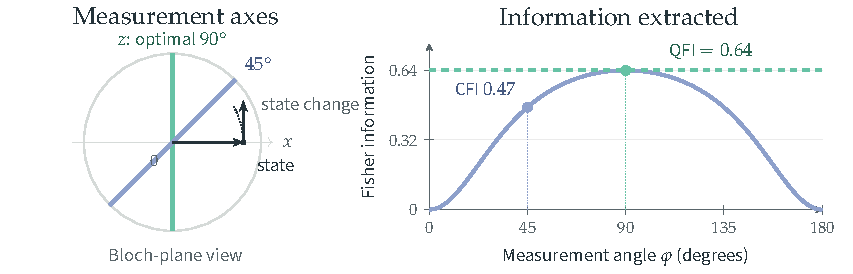
\includegraphics[width=14.1cm,height=4.35cm,keepaspectratio]{measurement_sensitivity.pdf}};
        \closingline{Changing the measurement raises CFI up to the quantum limit set by the state family.}
        \source{Exact illustration: Bloch radius $r=0.8$, local estimation of rotation $\theta$ (radians) at $\theta=0$. Derivation: Appendix J.}
        \footer{3 / 14}
    \end{canvas}
\end{frame}

\begin{frame}[plain,label=vqse]
    \begin{canvas}
        \heading{1\quad Information and variational estimation}{Variational spectral estimation}{Variational Quantum State Eigensolver (VQSE): a trainable spectral decomposition.}
        \wash{Blue}{.85}{6.17}{7.65}{3.91}
        \wash{Green}{7.9}{6.17}{15.15}{3.91}
        \node[txt,font=\rmfamily\large] at (1.15,5.85) {PCA: covariance matrix};
        \node[eq] at (1.15,5.25) {$C=\sum_i s_i\bm v_i\bm v_i^{\mathsf T}$};
        \node[smalltxt,text width=6cm] at (1.15,4.48) {Directions ranked by variance.};
        \node[txt,font=\rmfamily\large] at (8.2,5.85) {VQSE: density matrix};
        \node[eq] at (8.2,5.25) {$\rho=\sum_i\lambda_i\proj{v_i}$};
        \node[smalltxt,text width=6.55cm] at (8.2,4.48) {Components ranked by probability weight.};
        \node[eq] at (1.15,3.3) {$V(\bm\alpha)\rho V^\dagger(\bm\alpha)\approx\operatorname{diag}(\lambda_1,\lambda_2,\ldots)$};
        \node[txt,text width=14cm] at (1.15,2.43) {Frequencies estimate $\lambda_i$; the inverse rotation $V^\dagger\ket{i}$ recovers eigenvectors.};
        \closingline{Implemented VQSE supplies spectral information for fidelity-based QFI bounds.}
        \source{Cerezo et al., npj Quantum Information 8, 113 (2022); Beckey et al., Phys. Rev. Research 4, 013083 (2022).}
        \footer{4 / 14}
    \end{canvas}
\end{frame}

\begin{frame}[plain,label=qng]
    \begin{canvas}
        \heading{1\quad Information and variational estimation}{QFI geometry for variational optimization}{Circuit controls $\bm\alpha$ define an ansatz state family $\rho_{\bm\alpha}$.}
        \node[txt,text width=14cm] at (.95,6.1) {For an objective $C(\bm\alpha)$, account for how each control changes the state.};
        \wash{Blue}{.85}{5.26}{7.73}{2.5}
        \wash{Green}{7.97}{5.26}{15.15}{2.5}
        \node[txt,font=\rmfamily\large] at (1.15,4.96) {Newton's method};
        \node[eq] at (1.15,4.28) {$\Delta\bm\alpha=-\eta H_C^{-1}\nabla C$};
        \node[smalltxt,text width=6.18cm] at (1.15,3.34) {$H_C=\nabla^2C$\newline Curvature of the objective.};
        \node[txt,font=\rmfamily\large] at (8.27,4.96) {Quantum natural gradient};
        \node[eq,font=\fontsize{15}{19}\selectfont] at (8.27,4.28) {$\Delta\bm\alpha=-\eta(F^{\rm ans}+\lambda I)^{-1}\nabla C$};
        \node[smalltxt,text width=6.18cm] at (8.27,3.34) {Ansatz QFIM $F^{\rm ans}$\newline Distinguishability of neighbouring states.};
        \closingline{QNG preconditions the gradient with state geometry rather than the objective Hessian.}
        \source{Thesis: Mathematical Background; VQSE. $\lambda>0$ regularizes QNG; Newton expression assumes an invertible Hessian.}
        \footer{5 / 14}
    \end{canvas}
\end{frame}

\begin{frame}[plain,label=tfim]
    \begin{canvas}
        \heading{2\quad A finite quantum magnetometer}{Preparation and restricted access in the Ising model}{Six interacting spins encode the transverse field; measurements access four of them.}
        \foreach \i in {0,...,5}{
                \pgfmathsetmacro{\ang}{90-60*\i}
                \coordinate (q\i) at ({3.18+1.31*cos(\ang)},{4.43+1.31*sin(\ang)});
            }
        \draw[Rule,line width=2pt] (q0)--(q1)--(q2)--(q3)--(q4)--(q5)--cycle;
        \foreach \i in {0,...,3}{\fill[Green] (q\i) circle (.2);}
        \foreach \i in {4,5}{\draw[Muted,dashed,line width=.8pt] (q\i) circle (.2);}
        \node[smalltxt,text width=5cm,align=center] at (.7,2.78) {$N=6$\quad $n=4$ accessible spins\newline Periodic boundaries};
        \node[eq] at (6.25,6.0) {$H(h_x)=-J\sum_j Z_jZ_{j+1}-h_x\sum_j X_j$};
        \node[txt,font=\rmfamily\large] at (6.25,4.86) {Two preparation families};
        \node[eq,font=\fontsize{14}{18}\selectfont] at (6.25,4.16)
        {$\rho_{\rm G}=\proj{\psi_0(h_x)},\qquad \rho_\beta=\frac{e^{-\beta H(h_x)}}{Z_\beta}$};
        \node[txt,text width=8.5cm] at (6.25,3.03) {In both cases, the accessible state is\newline $\rho_S(h_x)=\Tr_E\rho(h_x)$.};
        \closingline{Compare the information in the same subsystem, across the same field range.}
        \source{Thesis: Noise Analysis, periodic $N=6$, $n=4$ preparation comparison. Gibbs preparation precedes partial trace.}
        \footer{6 / 14}
    \end{canvas}
\end{frame}

\begin{frame}[plain,label=thermal]
    \begin{canvas}
        \heading{2\quad A finite quantum magnetometer}{Thermal sensitivity beyond the ground-state optimum}{A lower peak can coexist with greater sensitivity away from the optimum.}
        \node[anchor=north west,inner sep=0pt] at (.63,6.12) {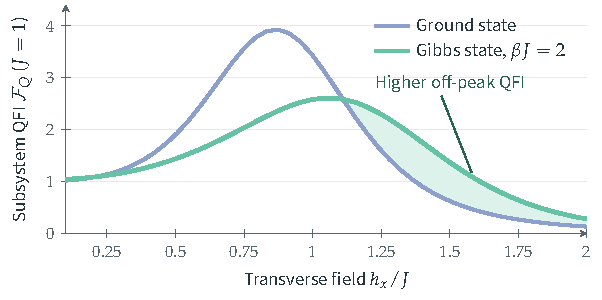
\includegraphics[width=10.5cm,height=4.5cm,keepaspectratio]{thermal_plot.pdf}};
        \draw[Rule] (11.26,5.98)--(11.26,2.12);
        \node[txt,font=\rmfamily\large,text width=3.45cm] at (11.62,5.73) {At $\beta J=2$};
        \node[txt,text width=3.45cm] at (11.62,4.95) {Peak QFI:\newline thermal $2.61$\newline ground state $3.93$};
        \node[txt,text width=3.45cm] at (11.62,3.42) {Higher sensitivity\newline away from the\newline ground-state peak.};
        \closingline{The preferred preparation depends on the expected field range as well as peak sensitivity.}
        \source{Exact SLD calculation; periodic $N=6$, $n=4$, $J=1$. Different preparation families; no universal thermal advantage.}
        \footer{7 / 14}
    \end{canvas}
\end{frame}

% Intentionally reserved for the user's detector photograph or schematic.
% Add \node[anchor=center] at (8,4.1) {\includegraphics[width=13.7cm,height=5.8cm,keepaspectratio]{spade_detector}};
% Keep this transition brief (approximately 10 seconds). No placeholder text is projected.
\begin{frame}[plain,label=spade-detector]
    \begin{canvas}
        \heading{3\quad An optical application: ASI Matera}{SPADE detector}{}
        \footer{8 / 14}
    \end{canvas}
\end{frame}

\begin{frame}[plain,label=record]
    \begin{canvas}
        \heading{3\quad An optical application: ASI Matera}{Spatial-mode measurements and the available record}{Spatial-mode sorting measures the displacement response of a faint companion.}
        \node[txt,font=\rmfamily\large] at (.95,6.08) {Physical measurement};
        \node[flow,draw=Green,line width=1pt] (sorter) at (2.4,4.71) {Spatial-mode\\ sorter};
        \draw[arr] (sorter.east)--(4.49,5.22);
        \draw[arr] (sorter.east)--(4.49,4.36);
        \node[txt,text width=2.6cm,font=\small] at (4.7,5.44) {$HG_{00}$\newline Reference mode};
        \node[txt,text width=2.6cm,font=\small] at (4.7,4.17) {$HG_{01},HG_{10}$\newline First-order modes};
        \node[smalltxt,text width=6.1cm] at (.95,2.76) {A choice of optical basis, before the data are recorded.};
        \draw[Rule] (7.68,6.05)--(7.68,2.14);
        \node[txt,font=\rmfamily\large] at (8.13,6.08) {Archived observations};
        \node[eq,font=\fontsize{16}{20}\selectfont] at (8.13,5.39) {$n_1=n_{HG_{01}}+n_{HG_{10}}$};
        \node[txt,text width=6.65cm] at (8.13,4.5) {525 settings $\times$ 100 repetitions\newline 52,500 counts; $10\,\mathrm{ms}$ per repetition};
        \node[smalltxt,text width=6.65cm] at (8.13,3.32) {Missing: resolved and failure outputs;\newline incident-flux monitoring;\newline measurements in additional bases.};
        \closingline{The record constrains the classical response; it does not identify the full optical state.}
        \source{Thesis: Quantum Channel Model for SPADE. Experiment: Santamaria, Sgobba and Lupo, Optica Quantum 2, 46--56 (2024).}
        \footer{9 / 14}
    \end{canvas}
\end{frame}



\begin{frame}[plain,label=sequence]
    \begin{canvas}
        \heading{3\quad An optical application: ASI Matera}{A quantum-to-classical channel model}{A physical forward model for propagation, measurement and detector reporting.}
        \node[flow,minimum height=1.5cm] (s) at (2.07,5.32) {Source state\\ $\rho_S$};
        \node[flow,minimum height=1.5cm,draw=Green,line width=1pt] (e) at (5.06,5.32) {Optical channel\\ $\mathcal E$};
        \node[flow,minimum height=1.5cm,draw=Blue,line width=1pt] (m) at (8.05,5.32) {Measurement\\ $\{M_y\}$};
        \node[flow,minimum height=1.5cm,draw=Orange,line width=1pt] (r) at (11.04,5.32) {Readout\\ $R$};
        \node[flow,minimum height=1.5cm] (n) at (14.03,5.32) {Repeated\\ counts};
        \draw[arr] (s)--(e);\draw[arr] (e)--(m);\draw[arr] (m)--(r);\draw[arr] (r)--(n);
        \node[eq,font=\fontsize{17}{21}\selectfont] at (2.15,4.18)
        {$p_y=\Tr\!\left[M_y\,\mathcal E(\rho_S)\right],\qquad \bm p_{\rm rep}=R\bm p$};
        \wash{Green}{.85}{3.38}{7.77}{2.05}
        \wash{Orange}{8.02}{3.38}{15.15}{2.05}
        \node[txt,text width=6.25cm,font=\small] at (1.15,3.15) {Quantum stages\newline Loss, dephasing and coherent mixing.};
        \node[txt,text width=6.5cm,font=\small] at (8.32,3.15) {Classical stages\newline Readout, calibration and count noise.};
        \closingline{The framework preserves physical constraints and locates losses of information.}
        \source{Thesis: sequential channel model. Coherence and optical-channel parameters are not reconstructed from aggregate counts.}
        \footer{10 / 14}
    \end{canvas}
\end{frame}

\begin{frame}[plain,label=kraus]
    \begin{canvas}
        \heading{3\quad An optical application: ASI Matera}{Kraus representations are not unique}{Different operator sets can describe exactly the same quantum channel.}
        \node[eq] at (1.18,6.01)
        {$\mathcal E(\rho)=\sum_aK_a\rho K_a^\dagger,\qquad \sum_aK_a^\dagger K_a=I$};
        \node[smalltxt,text width=14cm] at (1.18,5.16) {Example: complete dephasing of a two-mode state in the chosen basis.};
        \wash{Blue}{.85}{4.62}{7.75}{2.93}
        \wash{Green}{8.0}{4.62}{15.15}{2.93}
        \node[txt,font=\rmfamily\large] at (1.17,4.33) {Basis projectors};
        \node[eq,font=\fontsize{14}{18}\selectfont] at (1.17,3.9) {$K_0=\proj{0},\qquad K_1=\proj{1}$};
        \node[txt,font=\rmfamily\large] at (8.32,4.33) {Random phase flips};
        \node[eq,font=\fontsize{15}{19}\selectfont] at (8.32,3.9) {$\widetilde K_0=\frac{I}{\sqrt2},\qquad\widetilde K_1=\frac{Z}{\sqrt2}$};
        \node[eq,font=\fontsize{14}{18}\selectfont] at (1.18,2.64)
        {$\sum_aK_a\rho K_a^\dagger=\frac{\rho+Z\rho Z}{2}=\operatorname{diag}(\rho)$};
        \closingline{Kraus freedom changes the representation. Physical hypotheses concern the channel.}
        \source{Two-mode illustration of the thesis HG-dephasing model at $v=0$. Equivalent representations cannot be distinguished by system-only data.}
        \footer{11 / 14}
    \end{canvas}
\end{frame}

\begin{frame}[plain,label=loss]
    \begin{canvas}
        \heading{3\quad An optical application: ASI Matera}{A physical construction: mode-dependent loss}{Mode transmission $0\leq\tau_j\leq1$; loss is represented by an orthogonal failure state.}
        \node[txt,font=\rmfamily\large] at (.95,6.07) {Choose operators with explicit physical roles};
        \node[eq,font=\fontsize{16}{20}\selectfont] at (1.16,5.28)
        {$K_{\rm t}=\sum_j\sqrt{\tau_j}\proj{j},\qquad K_j^{\rm f}=\sqrt{1-\tau_j}\ket{\mathrm{fail}}\bra{j}$};
        \node[smalltxt,text width=14cm] at (1.16,4.37) {Transmission and failure jointly account for every input photon.};
        \wash{Green}{.85}{3.82}{15.15}{2.02}
        \node[eq,font=\fontsize{16}{20}\selectfont] at (1.16,3.5)
        {$K_{\rm t}^\dagger K_{\rm t}+\sum_j(K_j^{\rm f})^\dagger K_j^{\rm f}=\sum_j[\tau_j+(1-\tau_j)]\proj{j}=I$};
        \node[txt,text width=13.45cm] at (1.16,2.65) {Kraus form ensures complete positivity; completeness proves trace preservation.};
        \closingline{Channel validity can be proved mathematically; physical suitability requires calibration.}
        \source{Derived from the thesis mode-dependent loss map. Input: one-photon mode space after common survival; failure is retained in the output.}
        \footer{12 / 14}
    \end{canvas}
\end{frame}

\begin{frame}[plain,label=retention]
    \begin{canvas}
        \heading{3\quad An optical application: ASI Matera}{Information retained by the optical receiver}{Compare quantum and classical information at successive stages of the receiver.}
        \node[eq,font=\fontsize{16}{20}\selectfont] at (1.01,6.0)
        {$\mathcal F_Q(\rho_S)\;\geq\;\mathcal F_Q\!\left[\mathcal E(\rho_S)\right]\;\geq\;\mathcal F_C(\bm p)\;\geq\;\mathcal F_C(R\bm p)$};
        \node[smalltxt,text width=14cm] at (1.01,5.21) {For channels and measurements independent of the parameter being estimated.};
        \node[txt,font=\rmfamily\large] at (1.01,4.43) {Checkpoint};
        \node[txt,font=\rmfamily\large] at (10.78,4.43) {Fraction of source QFI};
        \draw[Rule] (1.01,3.93)--(15.0,3.93);
        \fill[Green] (1.02,3.4) circle (.075);
        \node[txt,text width=9.0cm] at (1.25,3.59) {Resolved reference, first-order and failure outputs};
        \node[txt,font=\fontsize{16}{20}\selectfont] at (10.78,3.62) {$99.68$--$100\%$};
        \draw[Rule] (1.01,2.99)--(15.0,2.99);
        \fill[Orange] (1.02,2.45) circle (.075);
        \node[txt,text width=9.0cm] at (1.25,2.65) {Binary readout; assumed $0.35\%$ port confusion};
        \node[txt,font=\fontsize{16}{20}\selectfont] at (10.78,2.68) {$0.13$--$57.0\%$};
        \closingline{Aggregation and readout confusion can strongly reduce the accessible information.}
        \source{Conditional model: same nine settings, per photon surviving common loss. Ranges across settings; not reconstructed experimental QFI.}
        \footer{13 / 14}
    \end{canvas}
\end{frame}

\begin{frame}[plain,label=conclusions]
    \begin{canvas}
        \heading{4\quad Conclusions}{From state information to experimental access}{Sensitivity depends on preparation, accessible degrees of freedom and measurement.}
        \fill[Blue] (.88,5.91) circle (.075);
        \node[txt,font=\rmfamily\large] at (1.16,6.1) {Variational estimation};
        \node[txt,text width=13.55cm] at (1.16,5.49) {Implemented spectral methods for mixed-state QFI bounds.\newline QFI geometry also provides a direction for circuit optimization.};
        \fill[Green] (.88,4.24) circle (.075);
        \node[txt,font=\rmfamily\large] at (1.16,4.43) {Preparation over a field range};
        \node[txt,text width=13.55cm] at (1.16,3.82) {Thermal preparation offers higher off-peak sensitivity in the studied regime.};
        \fill[Orange] (.88,2.95) circle (.075);
        \node[txt,font=\rmfamily\large] at (1.16,3.14) {A physically constrained observation model};
        \node[txt,text width=13.55cm] at (1.16,2.53) {Physical channels connect information limits to data and guide calibration.};
        \closingline{Next: resolved SPADE outputs, independent calibration and a programmable modal basis.}
        \source{QNG is a methodological connection; the optical variational protocol VQ-SPADE remains a proposal for a future experiment.}
        \footer{14 / 14}
    \end{canvas}
\end{frame}

\appendix

\begin{frame}[plain,noframenumbering,label=backup-bounds]
    \begin{canvas}
        \heading{Appendix A\quad Variational estimation}{Spectral truncation and the local-QFI limit}{Dominant eigencomponents bound a fidelity quantity at finite parameter displacement.}
        \node[eq] at (1.1,5.99) {$\displaystyle \mathcal I_\Delta=\frac{8[1-F(\rho_\theta,\rho_{\theta+\Delta})]}{\Delta^2}$};
        \node[txt,text width=13.6cm] at (1.1,4.62)
        {$F$ is root fidelity.\\[.3cm] The retained eigenspace is state dependent; it is not a fixed detector-mode cutoff.\\[.3cm] At regular operating points, $\mathcal I_\Delta\to\mathcal F_Q$ as $\Delta\to0$.};
        \closingline{Finite-step bounds need not be pointwise bounds on the exact SLD QFI.}
        \source{Thesis: Methods; Mathematical Background. Cerezo et al. (2022); Beckey et al. (2022).}
        \footer{Appendix A}
    \end{canvas}
\end{frame}

\begin{frame}[plain,noframenumbering,label=backup-qng]
    \begin{canvas}
        \heading{Appendix B\quad Variational optimization}{The ansatz metric and its scope}{The physical sensing parameter and the trainable circuit controls define different derivatives.}
        \node[eq,font=\fontsize{16}{20}\selectfont] at (1.03,5.96)
        {$F^{\rm ans}_{\mu\nu}=4\,\operatorname{Re}\!\left[\langle\partial_\mu\psi|\partial_\nu\psi\rangle
                    -\langle\partial_\mu\psi|\psi\rangle\langle\psi|\partial_\nu\psi\rangle\right]$};
        \node[txt,text width=13.7cm] at (1.03,4.98) {Pure ansatz: $F^{\rm ans}=4g_{\rm FS}$, the Fubini--Study metric up to convention.};
        \node[eq,font=\fontsize{13}{17}\selectfont] at (1.03,4.0)
        {$\displaystyle \min_{\Delta\bm\alpha}\;\nabla C^{\mathsf T}\Delta\bm\alpha
                +\frac{1}{2\eta}\Delta\bm\alpha^{\mathsf T}(F^{\rm ans}+\lambda I)\Delta\bm\alpha$};
        \node[txt,text width=13.7cm] at (1.03,2.77) {Stationarity gives the regularized natural-gradient update.\newline The quadratic term constrains state change, not objective curvature.};
        \closingline{Mixed VQSE inputs require a mixed-state metric; a pure-state metric is otherwise a surrogate.}
        \source{Thesis: Mathematical Background; VQSE. A full metric has quadratic parameter-count overhead; no general training speedup is claimed.}
        \footer{Appendix B}
    \end{canvas}
\end{frame}

\begin{frame}[plain,noframenumbering,label=backup-sr]
    \begin{canvas}
        \heading{Appendix C\quad Numerical optimization example}{Stochastic reconfiguration in a neural quantum state}{A separate pure-state RBM example illustrates metric-based optimization.}
        \node[anchor=north west,inner sep=0pt] at (1.5,6.14) {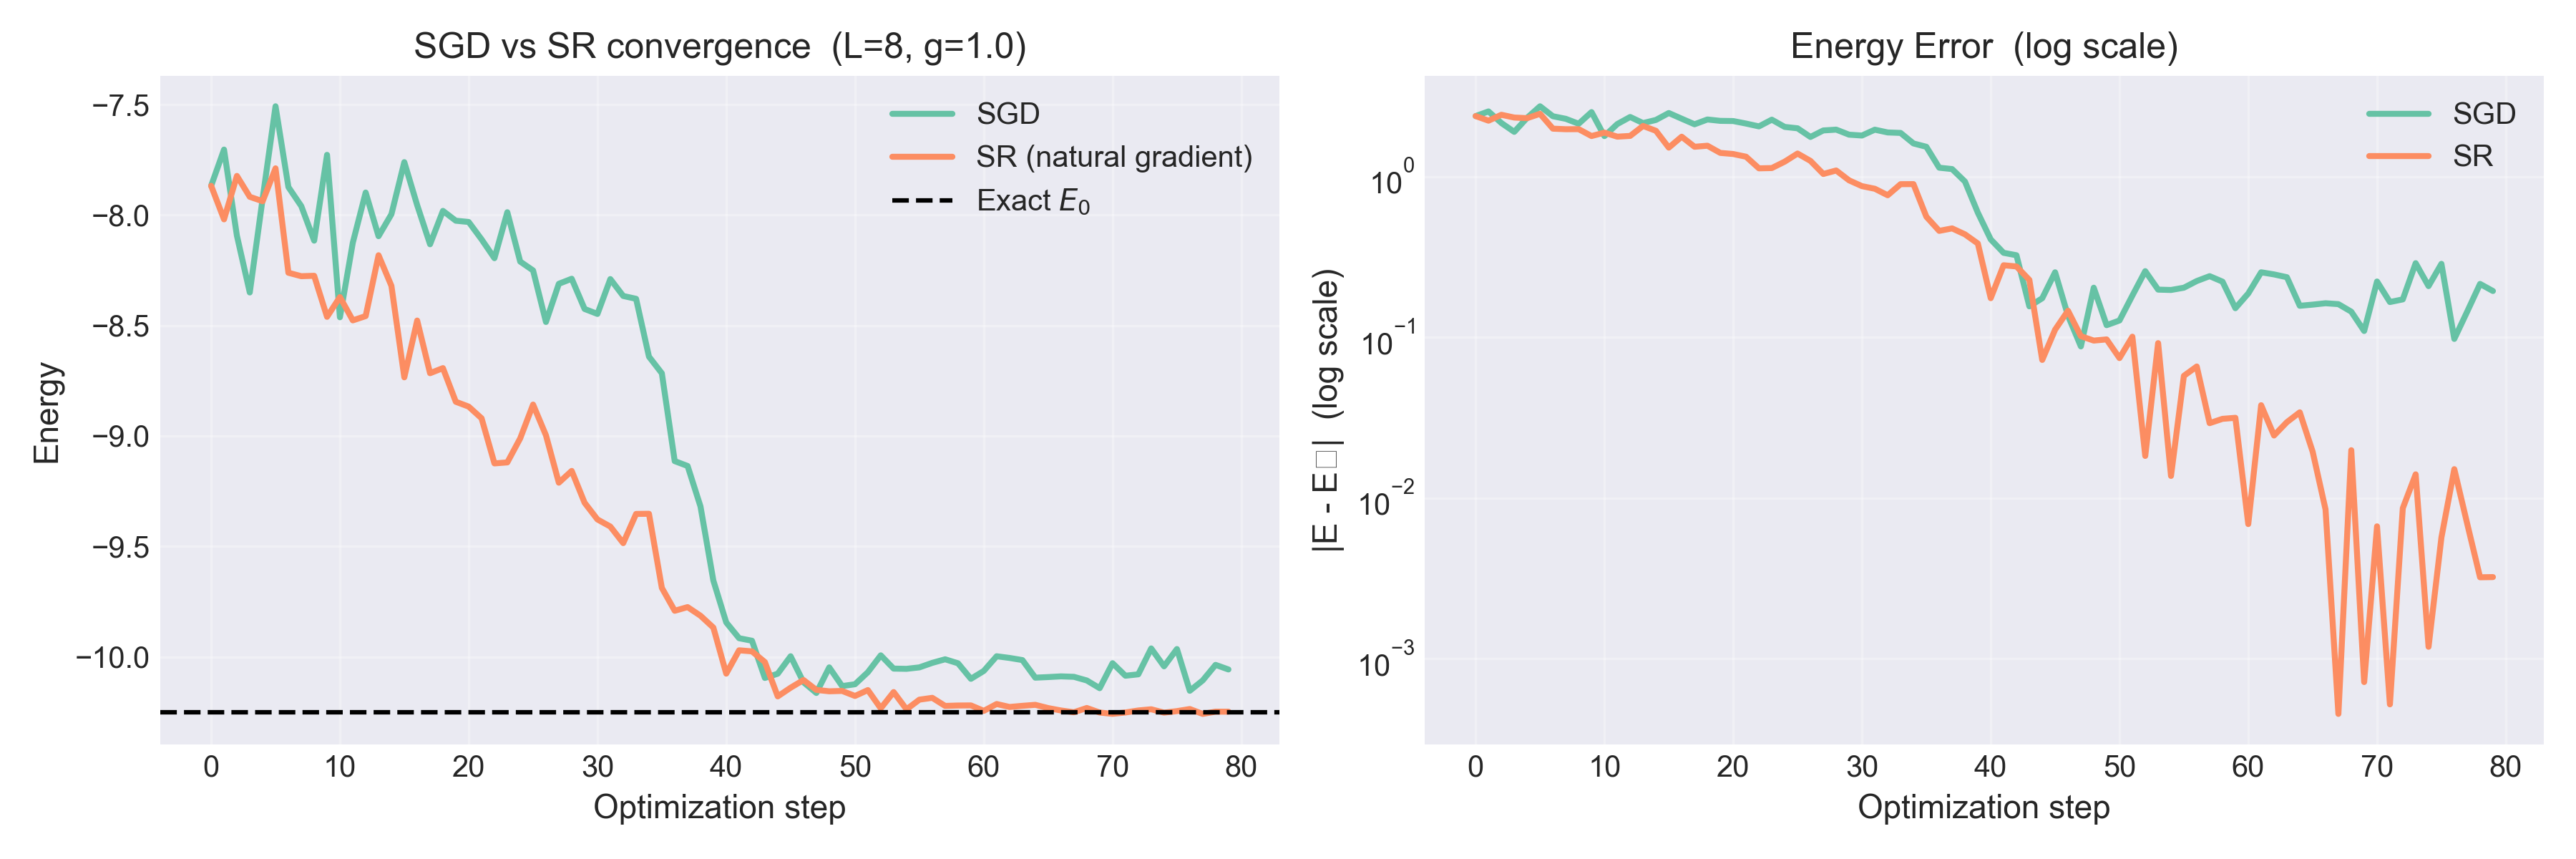
\includegraphics[width=13cm]{sr_comparison.png}};
        \closingline{SR lowers the energy error in this run; it does not benchmark mixed-state VQSE.}
        \source{Thesis figure: VQSE chapter. TFIM at $h_x/J=1$; 80 steps, 300 Monte Carlo samples/step, $\eta=0.05$, SR $\lambda=10^{-4}$; same seed.}
        \footer{Appendix C}
    \end{canvas}
\end{frame}

\begin{frame}[plain,noframenumbering,label=backup-thermal]
    \begin{canvas}
        \heading{Appendix D\quad Thermal preparation}{Thermal sensitivity and data processing}{The Gibbs and ground-state families need not have the same field response.}
        \node[eq] at (1.0,6.0) {$\rho_\beta(h_x)=\frac{e^{-\beta H(h_x)}}{\Tr e^{-\beta H(h_x)}}$};
        \node[txt,text width=13.8cm] at (1.0,4.85) {The field changes both eigenvectors and thermal populations.\newline Partial trace still obeys data processing within each family:};
        \node[eq] at (1.0,3.58) {$\mathcal F_Q[\Tr_E\rho_\beta(h_x)]\leq\mathcal F_Q[\rho_\beta(h_x)]$};
        \node[txt,text width=13.8cm] at (1.0,2.58) {For an uncertain field, choose an operating range or prior.\newline These curves do not establish a universal Bayesian or minimax optimum.};
        \closingline{The comparison changes the preparation family; it does not reverse a fixed noise channel.}
        \source{Thesis: Noise Analysis. Finite system; exact SLD QFI.}
        \footer{Appendix D}
    \end{canvas}
\end{frame}

\begin{frame}[plain,noframenumbering,label=backup-kraus]
    \begin{canvas}
        \heading{Appendix E\quad Channel representations}{Proof of Kraus-unitary freedom}{A change of Kraus basis leaves the channel unchanged.}
        \node[eq] at (1.0,5.96) {$\widetilde K_a=\sum_bu_{ab}K_b,\qquad U^\dagger U=I$};
        \node[eq,font=\fontsize{16}{20}\selectfont] at (1.0,4.76)
        {$\sum_a u_{ab}u_{ac}^*=\delta_{bc}$};
        \node[smalltxt] at (8.4,4.54) {Orthonormal columns of $U$.};
        \node[eq,font=\fontsize{13}{17}\selectfont] at (1.0,3.63)
        {$\sum_a\widetilde K_a\rho\widetilde K_a^\dagger
                =\sum_{b,c}\delta_{bc}K_b\rho K_c^\dagger
                =\sum_bK_b\rho K_b^\dagger$};
        \node[txt,text width=13.8cm] at (1.0,2.56) {Isometry in the Kraus index leaves the action on every input unchanged.};
        \closingline{A physical realization adds assumptions about the environment; the reduced map alone does not select them.}
        \source{Standard Kraus equivalence: an isometry, or a unitary after padding with zero operators. Algebra shown explicitly for this presentation.}
        \footer{Appendix E}
    \end{canvas}
\end{frame}

\begin{frame}[plain,noframenumbering,label=backup-embedding]
    \begin{canvas}
        \heading{Appendix F\quad Identifiability}{A classical response does not fix a quantum channel}{Embedding a stochastic map is a model construction, not process tomography.}
        \node[eq] at (1.0,6.0) {$\bm p\mapsto\operatorname{diag}(\bm p),\qquad \bm p'=R\bm p$};
        \node[txt,text width=13.8cm] at (1.0,5.1) {For a column-stochastic $R$, one valid quantum extension is};
        \node[eq] at (1.0,4.45) {$K_{ji}=\sqrt{R_{ji}}\ket{j}\bra{i},\qquad \mathcal E_R(\rho)=\sum_{ji}R_{ji}\rho_{ii}\proj{j}$};
        \node[txt,text width=13.8cm] at (1.0,3.34) {This extension measures and prepares in the chosen basis, erasing coherences.\newline For $R=I$, both the identity channel and complete dephasing reproduce the same populations.};
        \closingline{Different channels can agree on the measured populations; this is distinct from Kraus freedom of one channel.}
        \source{Thesis: classical/quantum embedding and HG coherence discussion. Channel-extension example derived for the presentation.}
        \footer{Appendix F}
    \end{canvas}
\end{frame}

\begin{frame}[plain,noframenumbering,label=backup-loss]
    \begin{canvas}
        \heading{Appendix G\quad Physical channel construction}{The loss map and its physical checks}{The input mode space is embedded in an output space containing an orthogonal failure flag.}
        \node[eq,font=\fontsize{16}{21}\selectfont] at (1.0,6.0)
        {$\mathcal L_{\bm\tau}(\rho)=K_{\rm t}\rho K_{\rm t}^\dagger
                +\Tr[(I-K_{\rm t}^\dagger K_{\rm t})\rho]\proj{\mathrm{fail}}$};
        \node[txt,text width=13.8cm] at (1.0,4.86) {For any ancillary system, Kraus form preserves positivity:\newline $\displaystyle (\mathcal L\otimes\mathrm{id})(X)=\sum_a(K_a\otimes I)X(K_a^\dagger\otimes I)\geq0$ for $X\geq0$.};
        \node[txt,text width=13.8cm] at (1.0,3.45)
        {Boundary checks: $\tau_j=1$ transmits mode $j$; $\tau_j=0$ sends it to failure.\newline Normalization: transmission plus failure has unit trace.\newline Physical validation: mode-injection measurements determine the $\tau_j$.};
        \closingline{Renormalizing the transmitted branch alone changes the question to postselected performance.}
        \source{Thesis: mode-dependent loss and flagged mode reduction. The record lacks independent modal-transmission calibration.}
        \footer{Appendix G}
    \end{canvas}
\end{frame}

\begin{frame}[plain,noframenumbering,label=backup-validation]
    \begin{canvas}
        \heading{Appendix H\quad Statistical validation}{Predictive calibration of the observed response}{A physical mean with a Gaussian-process correction predicts held-out setting means.}
        \node[eq,font=\fontsize{16}{20}\selectfont] at (1.0,6.0) {$\mu(d_a,\epsilon)=\mu_0(d_a,\epsilon)\exp[f(d_a,\epsilon)+\xi]$};
        \node[txt,text width=13.8cm] at (1.0,5.05) {Grouped five-fold validation; all components refitted within each training fold.};
        \node[txt,text width=14cm,font=\small] at (1.0,4.26) {
            \renewcommand{\arraystretch}{1.3}
            \begin{tabular}{lrrr}
                \toprule Held-out structure & RMSE  & Standardized SD & 95\% coverage \\\midrule
                Checkerboard cells          & 0.606 & 1.004           & 93.52\%       \\
                Distance rows               & 0.734 & 1.041           & 94.67\%       \\
                Source-ratio columns        & 0.609 & 1.009           & 93.71\%       \\\bottomrule
            \end{tabular}};
        \closingline{The validated target is the mean of 100 repetitions; this does not identify a complete quantum channel.}
        \source{Thesis: Exoplanet Experiment Appendix, hierarchical calibration validation. RMSE in counts per $10\,\mathrm{ms}$.}
        \footer{Appendix H}
    \end{canvas}
\end{frame}

\begin{frame}[plain,noframenumbering,label=backup-vqspade]
    \begin{canvas}
        \heading{Appendix I\quad Experimental outlook}{From SPADE to a variational optical measurement}{VQ-SPADE is a proposed optical realization of variational state eigensolving.}
        \node[eq,font=\fontsize{16}{21}\selectfont] at (1.0,6.0)
        {$p_k(\bm\alpha;d_a)=\bra{HG_k}V(\bm\alpha)\rho(d_a)V^\dagger(\bm\alpha)\ket{HG_k}$};
        \node[txt,text width=13.8cm] at (1.0,4.81)
        {A programmable coherent mode transformation provides the trainable basis.\\[.3cm] Resolved outputs, flux and failure events provide normalized probabilities.\\[.3cm] Nearby states and additional overlap measurements support fidelity-based QFI bounds.};
        \closingline{The present record motivates the acquisition design; it does not implement this protocol.}
        \source{Thesis: proposed VQ-SPADE scheme. Additional independent channel and background calibrations are required.}
        \footer{Appendix I}
    \end{canvas}
\end{frame}

\begin{frame}[plain,noframenumbering,label=backup-measurement]
    \begin{canvas}
        \heading{Appendix J\quad Measurement geometry}{An exact example of measurement-dependent CFI}{Unknown parameter: state rotation $\theta$. Measurement control: basis angle $\varphi$.}
        \node[eq,font=\fontsize{15}{19}\selectfont] at (1.0,6.0)
        {$\rho_\theta=\frac{I+r(\cos\theta\,X+\sin\theta\,Z)}{2},\qquad r=0.8$};
        \node[eq,font=\fontsize{14}{18}\selectfont] at (1.0,4.9)
        {$M_\pm^{(\varphi)}=\frac{I\pm(\cos\varphi\,X+\sin\varphi\,Z)}{2},\quad
                p_\pm=\frac{1\pm r\cos(\theta-\varphi)}{2}$};
        \node[eq,font=\fontsize{15}{19}\selectfont] at (1.0,3.74)
        {$\left.\mathcal F_C(\varphi)\right|_{\theta=0}
                =\frac{r^2\sin^2\varphi}{1-r^2\cos^2\varphi}\leq r^2=\mathcal F_Q$};
        \node[txt,text width=13.8cm] at (1.0,2.58)
        {At $\theta=0$, the SLD is $L_0=rZ$, so measuring $Z$ attains QFI.\newline The $45^\circ$ measurement gives $\mathcal F_C=8/17\simeq0.47$, compared with $\mathcal F_Q=0.64$.};
        \closingline{These directions label measurements for one parameter, not directions in a two-parameter QFIM.}
        \source{Derived from the CFI and SLD definitions in the thesis Mathematical Background. $r<1$ keeps this example full rank and regular.}
        \footer{Appendix J}
    \end{canvas}
\end{frame}

\end{document}
